\begin{center}
	\Large
	\textbf{BIOGRAFI PENULIS}
\end{center}

\addcontentsline{toc}{chapter}{BIOGRAFI PENULIS}

\vspace{2ex}

\begin{wrapfigure}{L}{0.3\textwidth}
	\centering
	\vspace{-3ex}
	% Ubah file gambar berikut dengan file foto dari mahasiswa
	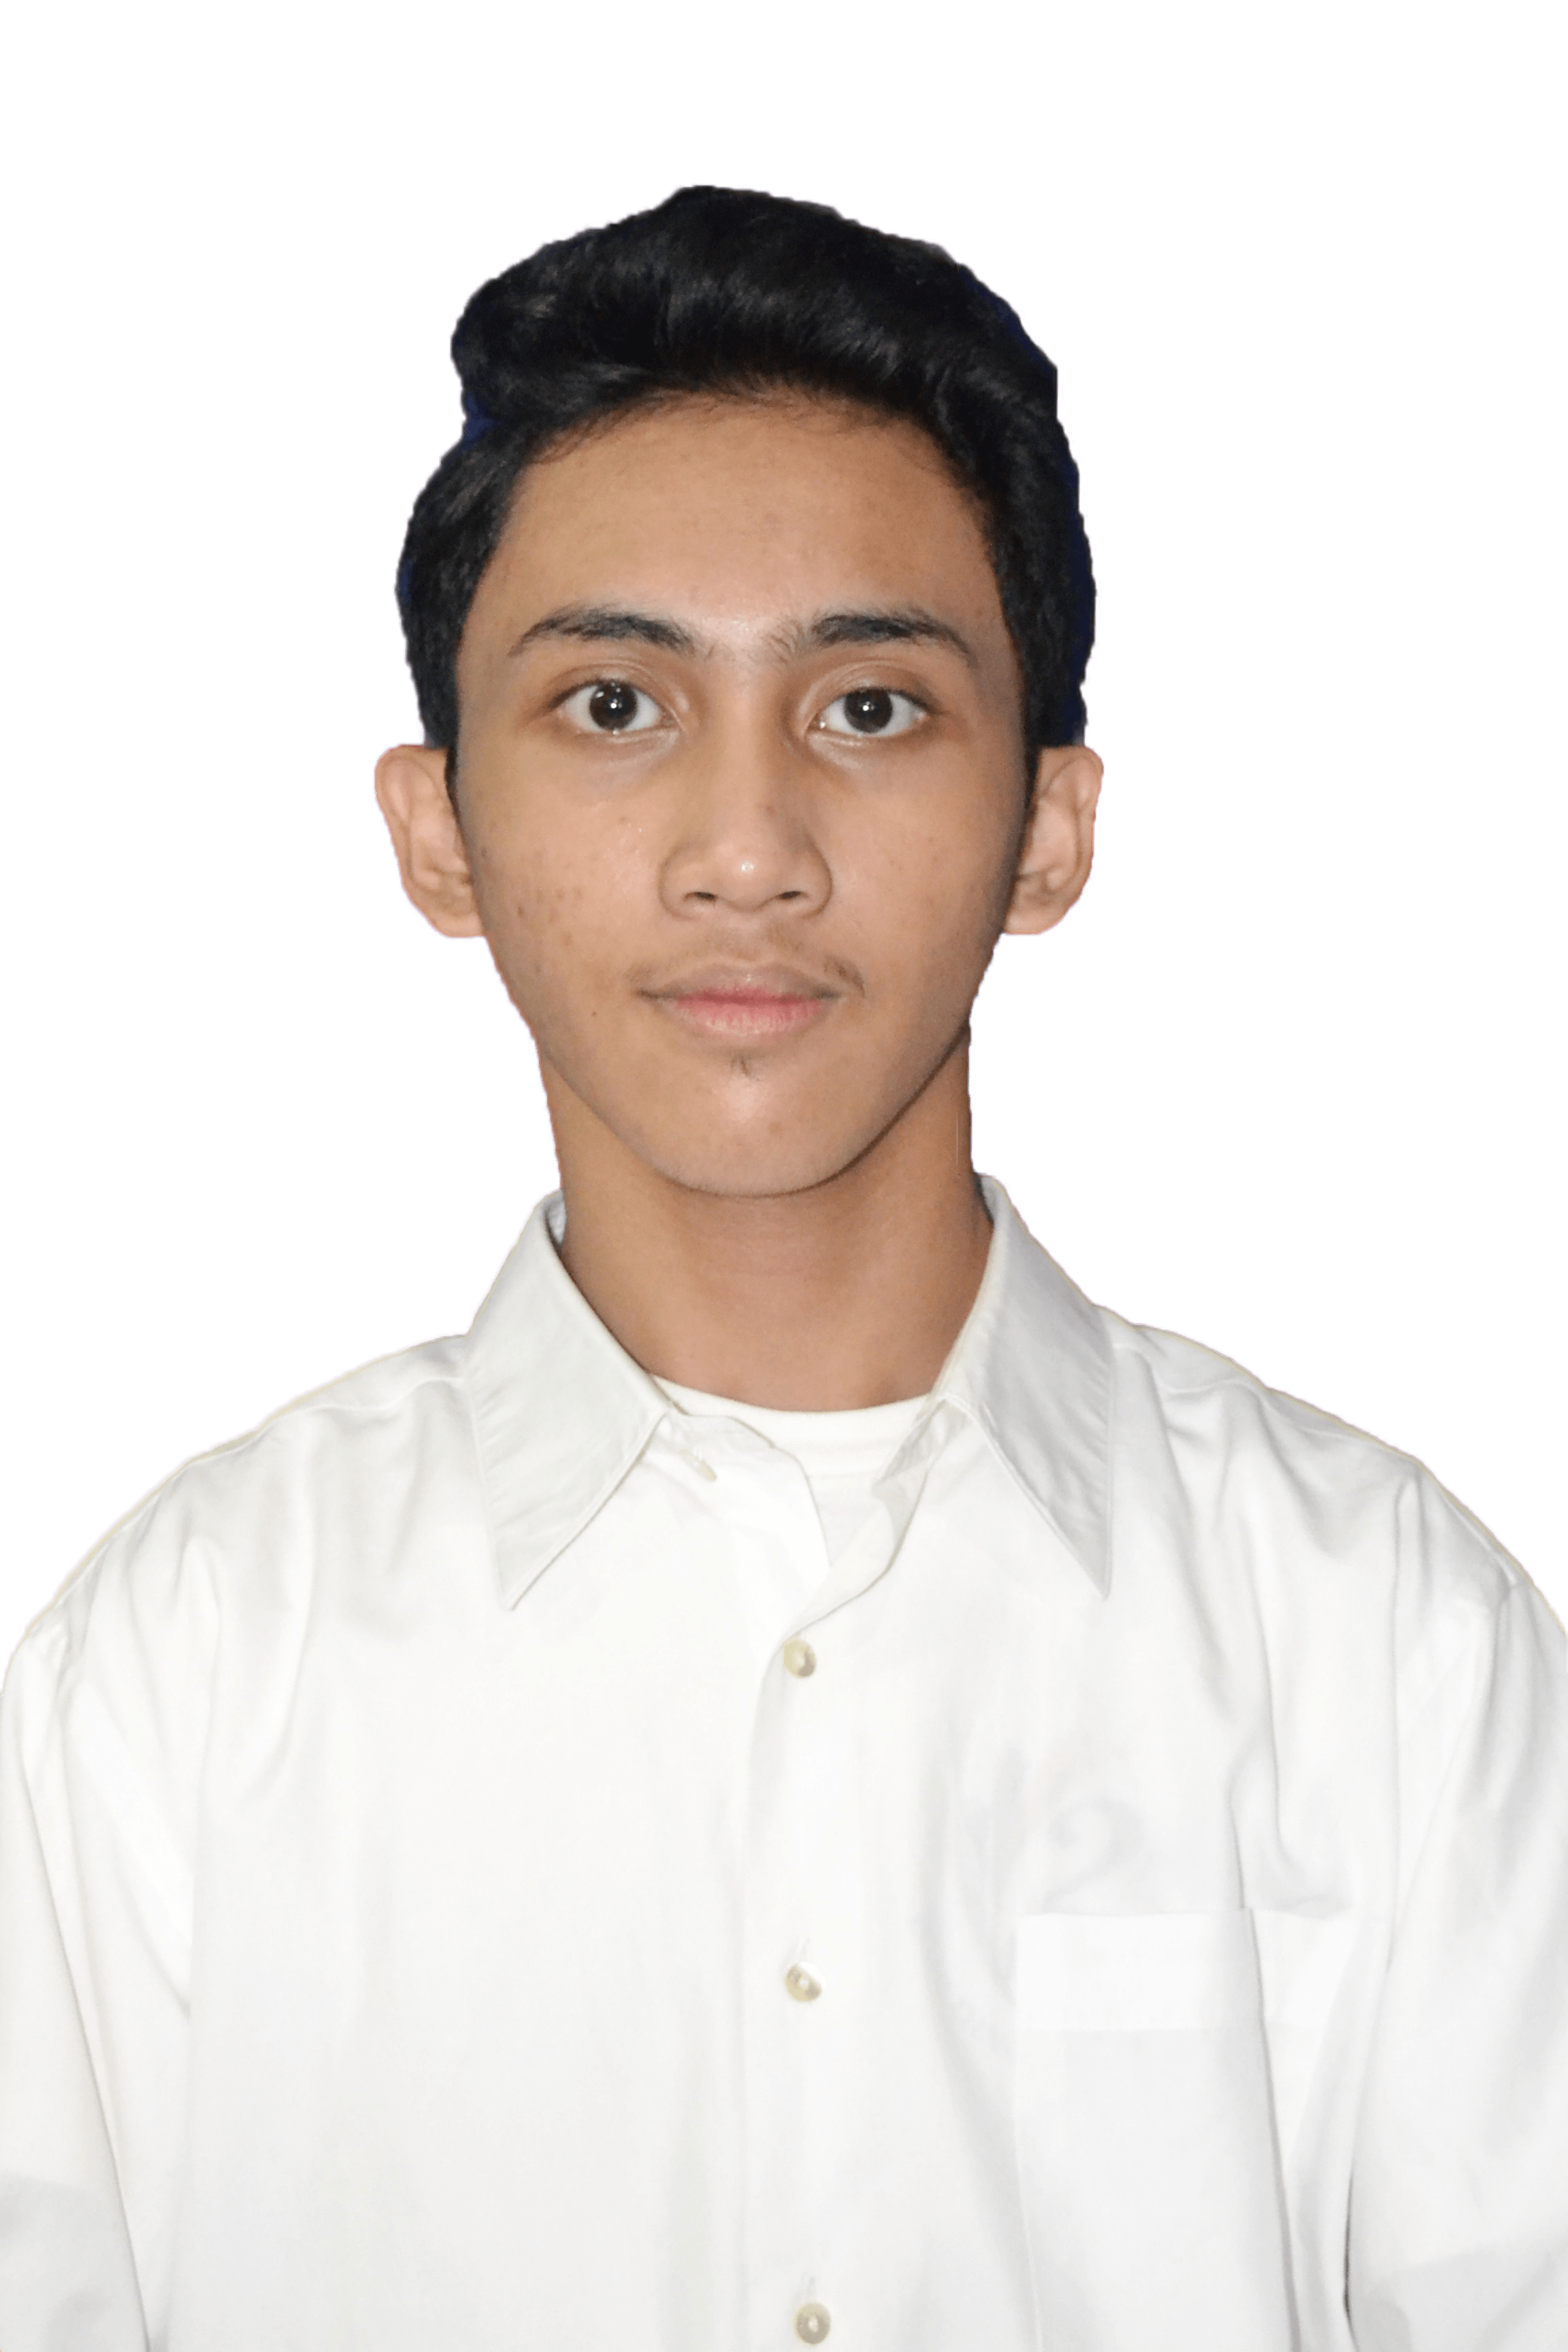
\includegraphics[width=0.3\textwidth]{BiografiPenulis/5024221026_Mahija Ibad Pradipta.png}
	\vspace{-4ex}
\end{wrapfigure}

% Ubah kalimat berikut dengan biografi dari mahasiswa
\name{}, atau yang biasa dikenal sebagai Mahija, lahir di Jakarta Pusat pada 7 Mei 2005. Penulis menyelesaikan pendidikan menengah di SMA Negeri 4 Jakarta sebelum melanjutkan studi ke jenjang strata satu di Departemen Teknik Komputer, Fakultas Teknologi Elektro dan Informatika Cerdas, Institut Teknologi Sepuluh Nopember (ITS) pada tahun 2022. Selama masa perkuliahan, penulis aktif sebagai asisten praktikum di Laboratorium Multimedia dan \textit{Internet of Things} (M-IoT) serta memiliki minat mendalam pada bidang \textit{embedded systems}, \textit{Internet of Things}, \textit{computer vision}, \textit{artificial intelligence}, robotika, dan \textit{edge computing}. Penulis juga memiliki pengalaman magang sebagai \textit{full-stack developer} di PT Winnicode Garuda Indonesia dan staf infrastruktur Jaringan IT di PT Lintasarta, serta berhasil meraih prestasi nasional pada Kontes Robot Bawah Air Indonesia (KRBAI) 2024 dan internasional di ajang Singapore Autonomous Underwater Vehicle Challenge (SAUVC) 2025. Dalam tugas akhir ini, penulis mengembangkan sistem drone otonom berbasis visi komputer untuk misi pencarian manusia. Penulis berharap penelitian ini bermanfaat bagi perkembangan teknologi \textit{Search and Rescue} (SAR) di Indonesia dan dapat dihubungi melalui surel mahijapradipta86@gmail.com.
